%!TEX encoding = UTF-8 Unicode

\documentclass [a4paper, 11pt, openany] {book}
\usepackage{verbatim}
%\usepackage{geometry}                % See geometry.pdf to learn the layout options. There are lots.
%\geometry{a4paper}                   % ... or a4paper or a5paper or ... 
%\geometry{landscape}                % Activate for for rotated page geometry
%\usepackage[parfill]{parskip}    % Activate to begin paragraphs with an empty line rather than an indent

%-----------------------------------------------------------------------------------------------------------------------*
%                                                                                                                       *
%   E N C O D A G E    D E S    S O U R C E S     :     U T F 8                                                         *
%                                                                                                                       *
%-----------------------------------------------------------------------------------------------------------------------*

%--- Paquetage pour le codage des sources en UTF-8
\usepackage[utf8]{inputenc}

%--- Latex demande ce paquetage pour mieux afficher le caractère "°" et \textquotesingle "'"
\usepackage{textcomp}

%--- Ce paquetage permet d'effectuer certaines césures, et ainsi d'éviter les messages "Overfull \hbox"
\usepackage[T1]{fontenc}

\usepackage{lmodern} % for French

\usepackage{filecontents}

%-----------------------------------------------------------------------------------------------------------------------*
%                                                                                                                       *
%   R É G L A G E S    « F R A N Ç A I S »                                                                              *
%                                                                                                                       *
%-----------------------------------------------------------------------------------------------------------------------*

%--- Paquetage pour imposer les réglages français
%\usepackage[francais]{babel}
\usepackage[frenchb]{babel}

%--- Contrôle de l'indentation et de la séparation des paragraphes
\setlength{\parindent}{0pt} 
%\setlength{\parskip}{1.2ex} % Reporté avant les chapitres

%--- Ajouter une séparation à la fin des itemize
\let\EndItemize\enditemize
\def\enditemize{\EndItemize\vspace{1.2ex}}

%-----------------------------------------------------------------------------------------------------------------------*
%                                                                                                                       *
%   M I S E    E N    P A G E                                                                                           *
%                                                                                                                       *
%-----------------------------------------------------------------------------------------------------------------------*

%--- Interligne 1,5 ligne
\usepackage{setspace}
\onehalfspacing

%--- Marge gauche : 2,8 cm ; le paramètre \hoffset contient cette valeur, moins 1 pouce
%    \hoffset = 2,8 cm - 2,54 cm = 0,26 cm
\setlength{\hoffset}{0.26 cm}

%--- Marges supplémentaires, différenciées pour les pages gauches et droites ; ici, aucune.
\setlength{\oddsidemargin }{0 cm}
\setlength{\evensidemargin}{0 cm}

%--- Largeur du texte
%    \textwidth = 210 mm - 28 mm - 28 mm = 15,4 cm
\setlength{\textwidth}{15.4 cm}

%--- Marge haute : 2,8 cm ; le paramètre \voffset contient cette valeur, moins 1 pouce
%    \voffset = 2,8 cm - 2,54 cm = 0,26 cm
\setlength{\voffset}{0.26 cm}

%--- Distance entre la marge haute et l'en-tête : 0 cm
\setlength{\topmargin}{0 cm}

%--- Hauteur de l'en-tête de chaque page : 1 cm
\setlength{\headheight}{1 cm}

%--- Distance entre l'en-tête de chaque page et le corps : 0,5 cm
\setlength{\headsep}{0.5 cm}

%--- Hauteur du corps
%    \textheight = 29,7 cm - 2,8 cm - 2,8 cm - 1,5 cm = 22,6 cm
\setlength{\textheight}{22.6 cm}

%-----------------------------------------------------------------------------------------------------------------------*
%                                                                                                                       *
%   T R A C E R    U N E    L I G N E    H O R I Z O N T A L E                                                          *
%                                                                                                                       *
%-----------------------------------------------------------------------------------------------------------------------*

\newcommand\ligne{\hrulefill}

%-----------------------------------------------------------------------------------------------------------------------*
%                                                                                                                       *
%   C H O I X    D E    L A    P O L I C E                                                                              *
%                                                                                                                       *
%-----------------------------------------------------------------------------------------------------------------------*

%---------------------------------------------------- Pour utiliser la police "Fourier"
%\usepackage{fouriernc}
%\usepackage[scaled=0.875]{helvet}

%\usepackage[scaled=0.8, default]{sourcesanspro}
\usepackage[scaled=0.9, default, semibold]{sourcecodepro}
\usepackage[default]{sourcesanspro}

%-----------------------------------------------------------------------------------------------------------------------*
%                                                                                                                       *
%   E X T E N S I O N S    P O U R    P R É S E N T E R    L E S    T A B L E A U X                                     *
%                                                                                                                       *
%-----------------------------------------------------------------------------------------------------------------------*

\usepackage{array}

%  http://en.wikibooks.org/wiki/LaTeX/Colors
\usepackage[dvipsnames, svgnames, table]{xcolor} % À placer avant \usepackage{listings}

%--- Ce paquetage permet de changer le style des légendes des tableaux et des figures (voir caption-eng.pdf) :
%  - l'étiquette est en italique gras
%  - le titre est en italique.
\usepackage[font=it, labelfont=bf]{caption}

%--- Par défaut, le paquetage nomme "Table" les tableaux. La commande
%   suivante impose le nom "Tableau"
% Voir http://fr.wikibooks.org/wiki/LaTeX/Éléments_flottants_et_figures
\addto\captionsfrench{\def\tablename{Tableau}}

%------------------------------------------------------------------------------------------ RÉFÉRENCES À UN TABLEAU
% La référence au tableau "nom-du-tableau" est définie par \labelTableau{nom-du-tableau}
\newcommand\labelTableau[1]{\label{tab:#1}}
% Latex autorise deux types d'appel à une référence \ref{tab:nom-du-tableau} et \pageref{tab:nom-du-tableau}

% \refTableau{}{nom-du-tableau} ---> "tableau x.y"   où x.y est le n° du tableau
\newcommand\refTableau[1]{\hyperref[tab:#1]{tableau \ref*{tab:#1}}}

% \refTableauSansPrefixe{}{nom-du-tableau} ---> "x.y"   où x.y est le n° du tableau
\newcommand\refTableauSansPrefixe[1]{\hyperref[tab:#1]{\ref*{tab:#1}}}

% \refTableauPage{}{nom-du-tableau} ---> "tableau x.y page n"   où x.y est le n° du tableau
\newcommand\refTableauPage[1]{\hyperref[tab:#1]{tableau \ref*{tab:#1} page \pageref{tab:#1}}}

% \refTableauPageSansPrefixe{}{nom-du-tableau} ---> "x.y page n"   où x.y est le n° du tableau
\newcommand\refTableauPageSansPrefixe[1]{\hyperref[tab:#1]{\ref*{tab:#1} page \pageref{tab:#1}}}

%-----------------------------------------------------------------------------------------------------------------------*
%                                                                                                                       *
%   T I K Z    -    P G F                                                                                               *
%                                                                                                                       *
%-----------------------------------------------------------------------------------------------------------------------*

\usepackage{tikz}
\usetikzlibrary{calc}
\usepackage{pgfplots}
\usetikzlibrary{arrows}
\usetikzlibrary{decorations}
\usetikzlibrary{decorations.pathmorphing}
\usetikzlibrary{shapes.callouts}
\usetikzlibrary{shapes.misc}
\usetikzlibrary{automata}
\usetikzlibrary{positioning}
\usepgflibrary{shapes.geometric}

%-----------------------------------------------------------------------------------------------------------------------*
%                                                                                                                       *
%   E N - T Ê T E S    E T    P I E D S    D E    P A G E S                                                             *
%                                                                                                                       *
%-----------------------------------------------------------------------------------------------------------------------*

% Grâce au package "fancyhdr"
% voir http://www.exomatik.net/U-Latex/Personnaliser#toc2
%      http://www.trustonme.net/didactels/250.html
\usepackage{fancyhdr}
\pagestyle{fancy}
%--- Numéro de page : à gauche pages paires, à droite pages impaires
\fancyhead[EL,OR]{\thepage}
%--- Nom de chapitre : à droite page paires
\fancyhead[ER]{\leftmark}
%--- Nom de section : à gauche page impaires
\fancyhead[OL]{\rightmark}
%--- Version : au milieu du pied de chaque page
\fancyfoot[C]{Easy Bindings}
%--- filet en haut et en bas de chaque page
\renewcommand{\headrulewidth}{0.5 pt}
\renewcommand{\footrulewidth}{0.5 pt}

\renewcommand{\chaptermark}[1]{\markboth{\bsc{\chaptername~\thechapter{}.} #1}{}}
\renewcommand{\sectionmark}[1]{\markright{\bsc{\thesection{}.} #1}{}}

%-----------------------------------------------------------------------------------------------------------------------*
%                                                                                                                       *
%   G E S T I O N    D E    L ' I N D E X                                                                               *
%                                                                                                                       *
%-----------------------------------------------------------------------------------------------------------------------*

% http://www.cuk.ch/articles/4097
% http://www.tuteurs.ens.fr/logiciels/latex/makeindex.html
% http://linux.die.net/man/1/makeindex
%
% Attention ! Les deux commandes suivantes, ainsi que le \printindex placé plus bas ne
% sont pas suffisants pour construire l'index : il faut utiliser l'utilitaire "makeIndex"
% Voir le fichier de commande "build.command"
\usepackage{makeidx}
\makeindex

%-----------------------------------------------------------------------------------------------------------------------*
%                                                                                                                       *
%   T O C B I D I N D                                                                                                   *
%                                                                                                                       *
%-----------------------------------------------------------------------------------------------------------------------*

%    Pour faire figurer la liste des tableaux (et la table des matières)
%    dans la table des matières
\usepackage{tocbibind}

\setcounter{tocdepth}{3}

%\titlespacing{\chapter} {0pt} {*0} {*0} {}
%\titlespacing{\section} {4ex} {*0} {*0} {}
%\titlespacing{\subsection} {10ex} {*0} {*0} {}
%\titlespacing{\subsubsection} {\subsubsectskip} {*0} {*0} {}

%\setlength{\parindent}{50pt}
%\makeatletter
%\renewcommand\paragraph{\@startsection{paragraph}{4}{\z@}%
%                                    {3.25ex \@plus 1ex \@minus .2ex}%
%                                    {2.3ex \ at plus.2ex}%
%                                    {\normalfont\normalsize\bfseries}}
%\makeatother

%-----------------------------------------------------------------------------------------------------------------------*
%                                                                                                                       *
%   H Y P E R R E F                                                                                                     *
%                                                                                                                       *
%-----------------------------------------------------------------------------------------------------------------------*

%--- Pour les hyperliens, et le contrôle de la génération PDF 
\usepackage{hyperref}
\hypersetup{colorlinks=true}
\hypersetup{linkcolor=blue}
\hypersetup{breaklinks=true}

%-----------------------------------------------------------------------------------------------------------------------*
%                                                                                                                       *
%   R É F É R E N C E S                                                                                                 *
%                                                                                                                       *
%-----------------------------------------------------------------------------------------------------------------------*

\usepackage{subfig}

%---- Nécessaire pour \refFigure...
\usepackage{ifthen}

% Au lieu d'écrire \chapter{titre-chapitre}, on écrit \chapterLabel{titre-chapitre}{label-chapitre}
\newcommand \chapterLabel[2]{\chapter{#1}\label{chapter:#2}}

% \refChapter{label-chapter} ---> "chapitre n"
\newcommand \refChapter[1]{\hyperref[chapter:#1]{chapitre \ref*{chapter:#1}}}

\newcommand \refChapterPage[1]{\hyperref[chapter:#1]{chapitre \ref*{chapter:#1} page \pageref{chapter:#1}}}

% Au lieu d'écrire \section{titre-section}, on écrit \sectionLabel{titre-section}{label-section}
\newcommand \sectionLabel[2]{\section{#1}\label{sec:#2}}


% \refSectionPage{label-section} ---> "section x.y page n"   où x.y est le n° de la section
\newcommand\refSectionPage[1]{\hyperref[sec:#1]{section \ref*{sec:#1} page \pageref{sec:#1}}}

%------------------------------------------------------------------------------------------ RÉFÉRENCES À UNE SUB-SECTION
% Au lieu d'écrire \subsection{titre-section}, on écrit \subsectionLabel{titre-section}{label-section}
\newcommand \subsectionLabel[2]{\subsection{#1}\label{subsec:#2}}


% \refSubsectionPage{label-section} ---> "section x.y page n"   où x.y est le n° de la sub-section
\newcommand\refSubsectionPage[1]{\hyperref[subsec:#1]{section \ref*{subsec:#1} page \pageref{subsec:#1}}}

%------------------------------------------------------------------------------------------ RÉFÉRENCES À UNE FIGURE
% La référence au tableau "nom-de-la-figure" est définie par \labelFigure{nom-de-la-figure}
\newcommand\labelFigure[1]{\label{fig:#1}}
% Latex autorise deux types d'appel à une référence \ref{fig:nom-de-la-figure} et \pageref{fig:nom-de-la-figure}

% \refFigure{}{nom-de-la-figure}   ---> "figure x.y"   où x.y est le n° de la figure
% \refFigure{z}{nom-de-la-figure}  ---> "figure x.y.z" où x.y est le n° de la figure
\newcommand\refFigure[2]{\hyperref[fig:#2]{figure \ref*{fig:#2}{\ifthenelse{\equal{#1}{}}{}{.#1}}}}

% \refFigureSansPrefixe{}{nom-de-la-figure}   ---> "x.y"   où x.y est le n° de la figure
% \refFigureSansPrefixe{z}{nom-de-la-figure}  ---> "x.y.z" où x.y est le n° de la figure
\newcommand\refFigureSansPrefixe[2]{\hyperref[fig:#2]{\ref*{fig:#2}{\ifthenelse{\equal{#1}{}}{}{.#1}}}}

% \refFigurePage{}{nom-de-la-figure}   ---> "figure x.y page n"   où x.y est le n° de la figure
% \refFigurePage{z}{nom-de-la-figure}  ---> "figure x.y.z page n" où x.y est le n° de la figure
\newcommand\refFigurePage[2]{\hyperref[fig:#2]{figure \ref*{fig:#2}{\ifthenelse{\equal{#1}{}}{}{.#1}} page \pageref{fig:#2}}}

% \refFigurePageSansPrefixe{}{nom-de-la-figure}   ---> "x.y page n"   où x.y est le n° de la figure
% \refFigurePageSansPrefixe{z}{nom-de-la-figure}  ---> "x.y.z page n" où x.y est le n° de la figure
\newcommand\refFigurePageSansPrefixe[2]{\hyperref[fig:#2]{\ref*{fig:#2}{\ifthenelse{\equal{#1}{}}{}{.#1}} page \pageref{fig:#2}}}

%-----------------------------------------------------------------------------------------------------------------------*
%                                                                                                                       *
%   E X T E N S I O N S    P O U R    L ' É C R I T U R E    D E S     F O R M U L E S    M A T H É M A T I Q U E S     *
%                                                                                                                       *
%-----------------------------------------------------------------------------------------------------------------------*

\usepackage{graphicx}
\usepackage{amssymb}
\usepackage{epstopdf}
\DeclareGraphicsRule{.tif}{png}{.png}{`convert #1 `dirname #1`/`basename #1 .tif`.png}

%-----------------------------------------------------------------------------------------------------------------------*
%   A F F I C H A G E    D U    C O D E    S H E L L                                                                    *
%-----------------------------------------------------------------------------------------------------------------------*

\newcommand\tpp[1]{\colorbox{gray!12}{\ttfamily #1}}

%-----------------------------------------------------------------------------------------------------------------------*
%                                                                                                                       *
%   C O D E   S O U R C E    S W I F T                                                                                  *
%                                                                                                                       *
%-----------------------------------------------------------------------------------------------------------------------*

\usepackage{listings}

\lstdefinelanguage{swift}
{
  morekeywords={
    func,if,then,else,for,in,while,do,switch,case,default,where,break,continue,fallthrough,return,
    typealias,struct,class,enum,protocol,var,func,let,get,set,willSet,didSet,inout,init,deinit,extension,
    subscript,prefix,operator,infix,postfix,precedence,associativity,left,right,none,convenience,dynamic,
    final,lazy,mutating,nonmutating,optional,override,required,static,unowned,safe,weak,internal,
    private,public,is,as,self,unsafe,dynamicType,true,false,nil,Type,Protocol,
  },
  morecomment=[l]{//}, % l is for line comment
  morecomment=[s]{/*}{*/}, % s is for start and end delimiter
  morestring=[b]" % defines that strings are enclosed in double quotes
}

\definecolor{keyword}{HTML}{BA2CA3}
\definecolor{string}{HTML}{D12F1B}
\definecolor{comment}{HTML}{008400}

\lstset{
  language=swift,
  basicstyle=\ttfamily,
  showstringspaces=false, % lets spaces in strings appear as real spaces
  columns=fixed,
  keepspaces=true,
  keywordstyle=\color{keyword},
  stringstyle=\color{string},
  commentstyle=\color{comment},
  frame=L,
}

%-----------------------------------------------------------------------------------------------------------------------*
%                                                                                                                       *
%   C O D E   S O U R C E    E A S Y - B I N D I N G S                                                                  *
%                                                                                                                       *
%-----------------------------------------------------------------------------------------------------------------------*

\usepackage{mdframed}

\newcommand\idfStyleEB[1]{\textcolor{gray}{#1}}
\newcommand\IdfStyleEB[1]{\textcolor{gray}{#1}}
\newcommand\bindingNameStyleEB[1]{\textcolor{orange}{#1}}

\newcommand\keywordsStyleEB[1]{\textcolor{blue}{\textbf{#1}}}
\newcommand\delimitersStyleEB[1]{\textcolor{brown}{\textbf{#1}}}
\newcommand\terminalStyleEB[1]{\textcolor{orange}{#1}}
\newcommand\nonTerminalStyleEB[1]{\textcolor{orange}{#1}}
\newcommand\integerStyleEB[1]{\textcolor{brown}{#1}}
\newcommand\floatStyleEB[1]{\textcolor{magenta}{#1}}
\newcommand\characterStyleEB[1]{\textcolor{cyan}{#1}}
\newcommand\stringStyleEB[1]{\textcolor{gray}{#1}}
\newcommand\typeNameStyleEB[1]{\textcolor{gray}{#1}}
\newcommand\attributeStyleEB[1]{\textcolor{brown}{#1}}
\newcommand\commentStyleEB[1]{\textcolor{red}{#1}}

%\newcommand\lexicalErrorEB{\textcolor{red}{\textbullet ERRLEX\textbullet}}

\newcommand\idfStyleeb[1]{\textcolor{gray}{#1}}
\newcommand\IdfStyleeb[1]{\textcolor{gray}{#1}}
\newcommand\bindingNameStyleeb[1]{\textcolor{orange}{#1}}

\newcommand\keywordsStyleeb[1]{\textcolor{blue}{\textbf{#1}}}
\newcommand\delimitersStyleeb[1]{\textcolor{brown}{\textbf{#1}}}
\newcommand\selectorStyleeb[1]{\textcolor{orange}{#1}}
\newcommand\terminalStyleeb[1]{\textcolor{orange}{#1}}
\newcommand\nonTerminalStyleeb[1]{\textcolor{orange}{#1}}
\newcommand\integerStyleeb[1]{\textcolor{brown}{#1}}
\newcommand\floatStyleeb[1]{\textcolor{magenta}{#1}}
\newcommand\characterStyleeb[1]{\textcolor{cyan}{#1}}
\newcommand\stringStyleeb[1]{\textcolor{gray}{#1}}
\newcommand\typeNameStyleeb[1]{\textcolor{gray}{#1}}
\newcommand\attributeStyleeb[1]{\textcolor{brown}{#1}}
\newcommand\commentStyleeb[1]{\textcolor{red}{#1}}

%\newcommand\lexicalErroreb{\textcolor{red}{\textbullet ERRLEX\textbullet}}

\newmdenv[
  topline=false,
  bottomline=false,
  rightline=false,
%  skipabove=\topsep,
%  skipbelow=\topsep,
  linecolor=blue!25,
  linewidth=2pt
]{siderules}

\newwrite\tempfile

\makeatletter
\newenvironment{ebcode}{%
  \begingroup
  \@bsphack
  \immediate\openout\tempfile=temp.eb%
  \let\do\@makeother\dospecials
  \catcode`\^^M\active
  \verbatim@startline
  \verbatim@addtoline
  \verbatim@finish
  \def\verbatim@processline{\immediate\write\tempfile{\the\verbatim@line}}%
  \verbatim@start
}{
  \immediate\closeout\tempfile
  \@esphack
  \endgroup
  \immediate\write18{eb --mode=latex:eb temp.eb}
  {\begin{siderules}\small\ttfamily\input{temp.eb.tex}\end{siderules}}
}
\makeatother

%-----------------------------------------------------------------------------------------------------------------------*
% COMMANDE \eb : affichage de code en ligne eb                                                                          *
%-----------------------------------------------------------------------------------------------------------------------*

\makeatletter
\newcommand*\eb{%
  \@bsphack%
  \begingroup%
  \let\do\@makeother\dospecials%
  \let\do\do@noligs\verbatim@nolig@list%
  \catcode`\^^M=15\relax%
  \@vobeyspaces%
  \@eb{\temporary}%
}%
\newcommand\@eb[2]{%
  \catcode`-=12\relax%
  \catcode`<=12\relax%
  \catcode`>=12\relax%
  \catcode`,=12\relax%
  \catcode`'=12\relax%
  \catcode``=12\relax%
  \catcode`#2\active%
  \catcode`~\active%
  \lccode`\~`#2\relax%
  \begingroup%
  \lowercase{%
    \def\@tempa##1~{%
      \expandafter\endgroup%
      \expandafter\DeclareRobustCommand%
      \expandafter*%
      \expandafter#1%
      \expandafter{\@tempa}%
      \@esphack%
      \immediate\openout\tempfile=temp.eb%
      \immediate\write\tempfile{##1}%
      \immediate\closeout\tempfile%
      \immediate\write18{eb --mode=latex:eb temp.eb}%
      \colorbox{gray!6}{\ttfamily\input{temp.eb.tex}\unskip}%
    }%
  }%
  \ifnum`#2=`\~\else\@makeother\~\fi%
  \expandafter\endgroup%
  \@tempa%
}%
\makeatother

%-----------------------------------------------------------------------------------------------------------------------*
%                                                                                                                       *
%   D É B U T    D U    D O C U M E N T                                                                                 *
%                                                                                                                       *
%-----------------------------------------------------------------------------------------------------------------------*


\begin{document} 

%-----------------------------------------------------------------------------------------------------------------------*
%                                                                                                                       *
%   P A G E    D E    T I T R E                                                                                         *
%                                                                                                                       *
%-----------------------------------------------------------------------------------------------------------------------*


\title{\Huge\bf Easy Bindings}
\author{Pierre Molinaro}
\date \today 
\maketitle

%-----------------------------------------------------------------------------------------------------------------------*
%                                                                                                                       *
%   T A B L E    D E S    M A T I È R E S                                                                               *
%                                                                                                                       *
%-----------------------------------------------------------------------------------------------------------------------*

\tableofcontents

%-----------------------------------------------------------------------------------------------------------------------*
%                                                                                                                       *
%   L I S T E    D E S    T A B L E A U X                                                                               *
%                                                                                                                       *
%-----------------------------------------------------------------------------------------------------------------------*

\listoftables
\addtocontents{lot}{\protect\thispagestyle{empty}\protect\pagestyle{empty}}

%-----------------------------------------------------------------------------------------------------------------------*
%                                                                                                                       *
%   L I S T E    D E S    F I G U R E S                                                                                 *
%                                                                                                                       *
%-----------------------------------------------------------------------------------------------------------------------*

\listoffigures
\addtocontents{lof}{\protect\thispagestyle{empty}\protect\pagestyle{empty}}

%-----------------------------------------------------------------------------------------------------------------------*
%                                                                                                                       *
%   L E S    C H A P I T R E S                                                                                          *
%                                                                                                                       *
%-----------------------------------------------------------------------------------------------------------------------*

%--- Contrôle de la séparation des paragraphes
%    On met cette définition ici, sinon elle affecte la table des matières, la liste des tableaux, ...
\setlength{\parskip}{1.2ex}

%!TEX encoding = UTF-8 Unicode
%!TEX root = ../easy-bindings.tex


\chapter{Tutorial}

\section{Introduction}

À partir de mac OS X 10.3 (Panther), le pattern MVC\index{MVC} (\emph{Model View Controller}) peut être mis en œuvre au moyen des \emph{Cocoa Bindings}. Ceux-ci ont perduré jusqu'aux systèmes actuels, et notamment peuvent actuellement être exprimés en Swift.

La technique préconisée par Apple pour exprimer le pattern MVC est d'écrire les \emph{bindings} directement dans l'interface graphique \emph{Interface Builder} de \emph{Xcode}. Cette approche, si elle est simple pour des petits programmes d'exemple, présente à notre avis plusieurs inconvénients pour des projets importants :
\begin{itemize}
  \item à la moindre erreur, le \emph{binding} ne fonctionne pas, ou assez souvent il en résulte un \emph{crash} de l'application ;
  \item suite à un changement de nom d'une propriété, il faut revoir tous les \emph{outlets} qui lui sont liés, en balayant les multiples items graphiques ;
  \item les valeurs transmises sont des objets Objective-C : les entiers, structures, énumérations sont convertis en instances de \texttt{NSNumber} ou de \texttt{NSValue}, les objets en instance de \texttt{NSObject}, perdant ainsi toute possibilité de vérification statique de la correction des types. 
\end{itemize}

Si tous ces points ne sont pas gênants pour un petit exemple, il s'avère en pratique que la maintenance d'une application comportant de nombreux \emph{bindings} est plus compliquée qu'il n'y paraît. Comme il n'y a pas de possibilité de vérification statique à la compilation, au moindre changement on doit s'astreindre à passer en revue dans \emph{Interface Builder} tous les \emph{outlets} : en pratique, il est fatal d'en oublier. L'erreur peut apparaître bien longtemps après la modification, si la fonction concernée n'est que peu utilisée.


\tpp{eb} est un outil facilitant la mise en œuvre du pattern MVC\index{MVC} (\emph{Model View Controller}) pour des applications Mac OS X écrites en Swift :
\begin{itemize}
  \item \emph{Interface Builder} est utilisé uniquement pour dessiner l'interface, et définir les \emph{outlets} ;
  \item aucune information de \emph{binding} n'apparaît dans \emph{Interface Builder} ;
  \item un texte \emph{Easy Bindings} est écrit pour définir les modèles et les bindings ;
  \item la compilation par l'outil \tpp{eb} de ce texte engendre du code \emph{Swift} prêt à être compilé.
\end{itemize}

Cet outil en fait va plus loin que la seule définition des \emph{bindings} :
\begin{itemize}
 \item il permet la définition des préférences ;
 \item il permet la définition des documents, y compris sauvegarde sur fichier et leur lecture ;
 \item le code engendré permet une vérification statique de la correction des bindings ;
 \item il engendre du code code qui à l'exécution maintient une liste des objets alloués, facilitant ainsi la bonne gestion des objets, notamment pour vérifier que la fermeture d'un document libère tous ses objets.
\end{itemize}

La génération du code \emph{Swift} par \tpp{eb} est effectuée de telle façon qu'elle conserve certaines modifications qui lui sont apportées : ainsi, en suivant quelques règles élémentaires, une regénération provoquée par une compilation des sources \emph{Easy Bindings} ne détruit pas le code ajouté à la main.

\section{Premier exemple : gestion des préférences}

\subsectionLabel{Texte source}{textSourceTutorialUn}

\begin{ebcode}
xcodeproject "fr.irccyn.molinaro" ;

mainxib {
  {"String:", EBTextField myTextField},
  {"String (send continously): ", EBTextField myOtherTextField},
  {"String observer:", EBTextObserverField myObserverTextField},
  {"Color:", EBColorWell mColorWell},
  {"Color (send continously):", EBColorWell mContinousColorWell},
  {"Color Observer:", EBColorObserverWell mObserverColorWell},
  {"Date:", EBDatePicker mDatePicker},
  {"Even Integer:", EBIntField mIntegerTextField},
  {"Even Integer Observer:", EBIntObserverField mIntegerObserverTextField}
}

prefs {
#--- String
  property String myString default "hello" ;
  outlet EBTextField myTextField $value self.myString {sendContinously : no} ;
  outlet EBTextField myOtherTextField $value self.myString {sendContinously : yes} ;
  outlet EBTextObserverField myObserverTextField $valueObserver self.myString ;
#--- Color
  property NSColor mColor default yellowColor ;
  outlet EBColorWell mContinousColorWell $color self.mColor {sendContinously : yes} ;
  outlet EBColorWell mColorWell $color self.mColor {sendContinously : no} ;
  outlet EBColorObserverWell mObserverColorWell $colorObserver self.mColor ;
#--- Date
  property NSDate mDate default date ;
  outlet EBDatePicker mDatePicker $date self.mDate  ;
#--- Number
  property validates Int mIntegerValue default 12 ;
  outlet EBIntField mIntegerTextField
    $value self.mIntegerValue {sendContinously : yes, autoFormatter:yes}
  ;
  outlet EBIntObserverField mIntegerObserverTextField
    $valueObserver self.mIntegerValue {autoFormatter:yes}
  ;
}
\end{ebcode}

Le texte source est divisé en trois parties :
\begin{itemize}
  \item génération d'un projet Xcode (clause \eb!xcodeproject!, \refSubsectionPage{clauseProject}) ;
  \item description de l'interface (clause \eb!mainxib!, \refSubsectionPage{clauseMainXIB}) ;
  \item description des préférences (clause \eb!prefs!, \refSubsectionPage{clausePrefs}).
\end{itemize}

La première partie (clause \eb!xcodeproject!) ordonne la génération d'un projet Xcode, ce qui est utile dans le cadre d'un petit programme d'exemple.  Dans un vrai projet, on préfèrera écrire le projet à la main.
 
La deuxième partie (clause \eb!mainxib!) permet de décrire une interface très sommaire, utile simplement pour un petit programme d'exemple, destiné à un tutorial comme celui-ci. Dans un vrai projet, on préfèrera écrire l'interface à la main.

La troisième partie (clause \eb!prefs!) est la définition des préférences, c'est-à-dire des propriétés (\eb!property!), et outlets (\eb!outlet!) et de leurs bindings (\eb!$value!),  (\eb!$valueObserver!), ...






\subsection{Compilation du texte source}

Le code ci-dessus (\refSubsectionPage{textSourceTutorialUn}) doit être contenu dans un fichier dont l'extension est \tpp{.eb}, par exemple \tpp{tutorial1.eb}. Pour le compiler, on peut utiliser l'outil en ligne de commande \tpp{eb}, ou l'application Mac OS X \tpp{CocoaEb} :

\tpp{eb tutorial1.eb}

Sont engendrés, dans le même répertoire que le fichier source :
\begin{itemize}
  \item un fichier projet Xcode : \tpp{tutorial1.xcodeproj} ;
  \item un répertoire \tpp{tutorial1} contenant tous les sources Swift et les fichiers d'interface graphique.
\end{itemize}

La compilation du projet Xcode fait apparaître plusieurs warnings :
\begin{itemize}
\item des warnings « \emph{Update to recommended settings} » et « \emph{This file is set to build for a version older than the deployment target. Functionality may be limited.} » que l'on peut ignorer pour ce programme d'exemple ;
\item le warning « \emph{Will never be executed} » qui désigne une portion de code inatteignable ; ce warning concerne un code qui doit être modifié à la main, la génération de ce warning est volontaire pour que l'utilisateur en soit averti ; il sera étudié à la \refSubsubsectionTitlePage{validationSaisie}.
\end{itemize}


\begin{figure}[t]
  \centering
  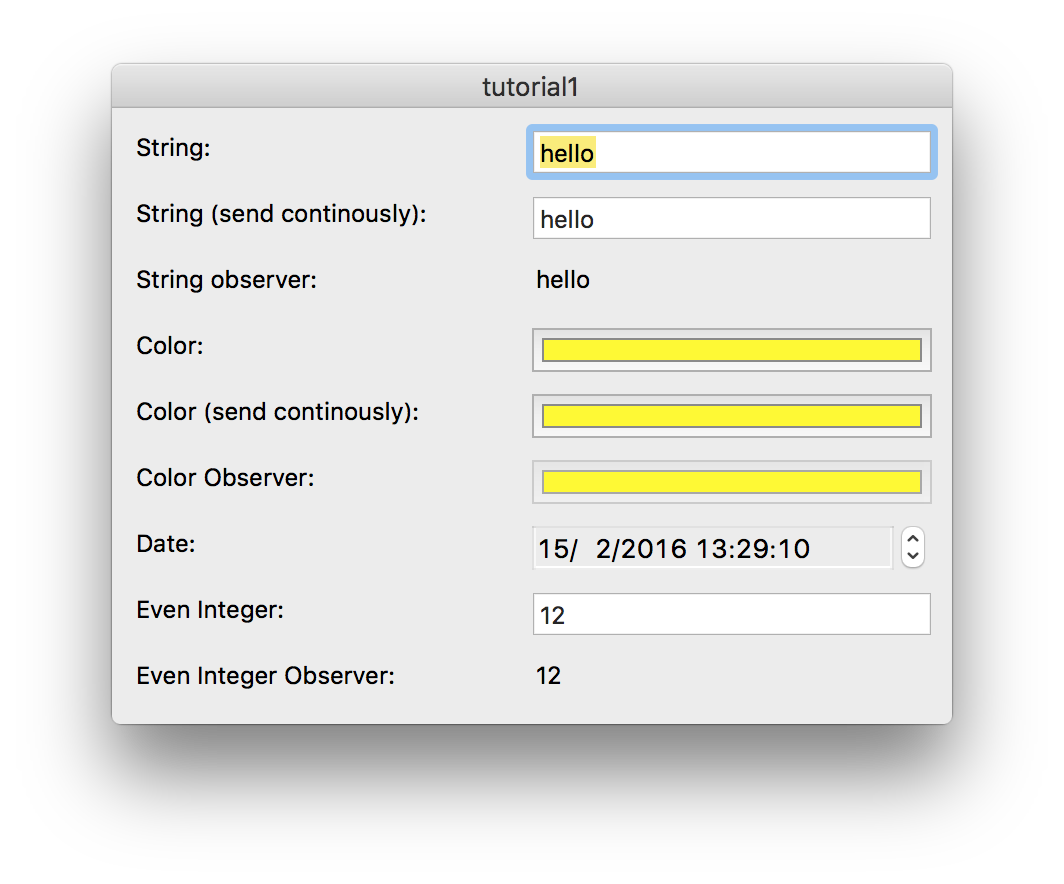
\includegraphics[width=8cm]{chapitres/tutorial1.png}
  \small
\begin{ebcode}
mainxib {
  {"String:", EBTextField myTextField},
  {"String (send continously): ", EBTextField myOtherTextField},
  {"String observer:", EBTextObserverField myObserverTextField},
  {"Color:", EBColorWell mColorWell},
  {"Color (send continously):", EBColorWell mContinousColorWell},
  {"Color Observer:", EBColorObserverWell mObserverColorWell},
  {"Date:", EBDatePicker mDatePicker},
  {"Even Integer:", EBIntField mIntegerTextField},
  {"Even Integer Observer:", EBIntObserverField mIntegerObserverTextField}
}
\end{ebcode}
  \caption{Interface graphique du premier tutorial et sa description}
  \labelFigure{interfaceGraphiquePremierTutorial}
  \ligne
\end{figure}

Après compilation Xcode, le projet est prêt à être exécuté ; le lancer fait apparaître la fenêtre illustrée par la \refFigurePage{}{interfaceGraphiquePremierTutorial}.

Les sections qui suivent sont consacrées à la description du texte source \emph{Easy Bindings}, en commençant par la clause \eb!mainxib!, suivie de la clause \eb!prefs!.







\subsectionLabel{Clause \texttt{xcodeproject}}{clauseProject}\index{xcodeproject}

La clause \eb!xcodeproject! permet d'ordonner la génération d'un projet Xcode. Le seul paramètre à fournir est la chaîne permettant de définir le « \emph{Bundle Identifier} » de l'application :
\begin{ebcode}
xcodeproject "fr.irccyn.molinaro" ;
\end{ebcode}

Le « \emph{Bundle Identifier} » de l'application est construit à partir de la chaîne fournie, en ajoutant un point suivi du nom du fichier source \emph{Easy Binding} sans son extension : pour le fichier \texttt{tutorial1.eb}, le « \emph{Bundle Identifier} » est \texttt{fr.irccyn.molinaro.tutorial1}.




\subsectionLabel{Clause \texttt{mainxib}}{clauseMainXIB}\index{mainxib}

La clause \eb!mainxib! permet de décrire une fenêtre liées aux \emph{préférences} de l'application. La présentation est systématique (\refFigurePage{}{interfaceGraphiquePremierTutorial}), deux colonnes, celle de gauche étant un commentaire, celle de droite contenant l'item graphique (bouton, champ texte, …). Ceci est uniquement destiné à réaliser rapidement des petits exemples illustratifs.

Le code est une description ligne par ligne de la composition de la fenêtre, en commençant par le haut ; Chaque ligne a la forme suivante : 
\begin{ebcode}
  {"commentaire", TypeOutlet nomOutlet}
\end{ebcode}

\eb!"commentaire"! est le texte qui est affiché dans la colonne de gauche ; \eb!TypeOutlet! et \eb!nomOutlet! sont évidemment le type et le nom de l'outlet. À noter que les types définis par Cocoa (\texttt{NSTextField}, \texttt{NSColorWell}, …) ne sont pas utilisés, au profit de types propres à \emph{Easy Bindings} : \eb!EBTextField!,  \eb!EBTextObserverField!, \eb!EBObserverWell!, \eb!EBColorObserverWell!, … La raison en est la suivante : les bindings d'\emph{Easy Bindings} nécessitent des propriétés complémentaires et un typage fort qui ne ne peuvent pas être exprimés directement avec les classes définies dans Cocoa ; les classes définies dans \emph{Easy Bindings} en héritent et implémentent les bindings.

{\bf Attention : } La vérification de la cohérence \eb!TypeOutlet! et \eb!nomOutlet! avec leur utilisation dans la clause \eb!prefs! n'est pas effectuée : une erreur n'est pas décelée lors de la compilation \emph{Easy Bindings}, et a des conséquences imprévisibles dans le projet Xcode : erreur de compilation, d'exécution, …










\subsectionLabel{Clause \texttt{prefs}}{clausePrefs}\index{prefs}

Une clause \eb!prefs! décrit modèles et bindings. Le seul couplage entre cette description et la description graphique (dans une classe \eb!mainxib! ou à la main) est constitué par les outlets et leur type. Sa compilation engendre un fichier \texttt{Preferences.swift} qui définit la classe \texttt{Preferences}.

%Un projet accepte zéro, une ou plusieurs clauses \eb!prefs! ; écrire :
%\begin{ebcode}
%prefs {
%  # définitions A
%}
%prefs {
%  # définitions B
%}
%prefs {
%  # définitions C
%}
%\end{ebcode}
%
%est équivalent à :
%\begin{ebcode}
%prefs {
%  # définitions A
%  # définitions B
%  # définitions C
%}
%\end{ebcode}

\subsubsection{Déclaration des propriétés}

Observons la première ligne de la clause \eb!prefs! (\refSubsectionPage{textSourceTutorialUn}) :
\begin{ebcode}
  property String myString default "hello" ;
\end{ebcode}

Elle déclare le modèle \eb!myString!, de type \eb!String!, dont la valeur initiale est \eb!"hello"!. Dans le code engendré, \texttt{myString} est une propriété de la classe \texttt{Preferences}. Son type est \texttt{EBStoredProperty\_String}. Cette classe prend complètement en charge l'écriture et la lecture de la valeur dans les préférences de l'application (la clef associée est \texttt{Preferences:myString}).

La valeur initiale n'est utilisée que lors du premier lancement de l'application, ou lorsqu'une propriété est ajoutée, c'est-à-dire quand la clé \texttt{Preferences:myString} n'existe pas dans les préférences de l'application.

Il en est de même pour les autres propriétés :
\begin{ebcode}
  property NSColor mColor default yellowColor ;
  ...
  property NSDate mDate default date ;
  ...
  property validates Int mIntegerValue default 12 ;
\end{ebcode}

La dernière déclaration fait apparaître le mot réservé \eb!validates! qui ordonne la validation des données saisie via l'interface ; ce point est examiné à la \refSubsubsectionTitlePage{validationSaisie}.


\subsubsection{Déclaration des outlets de leurs bindings}



\subsubsectionLabel{Validation de la saisie}{validationSaisie}



%!TEX encoding = UTF-8 Unicode
%!TEX root = ../easy-bindings.tex


\chapter{Structure globale}



L'entrée du compilateur EasyBindings est un fichier source. Celui-ci peut en inclure d'autres via une déclaration \fcolorbox{white}{green}{\bf include}. D'une manière générale, un fichier source contient une liste de \emph{déclarations} :
\begin{itemize}
  \item déclaration d'une classe d'outlet (\refSectionPage{declarationOutletClasse}) ;
  \item inclusion d'un autre fichier (\refSectionPage{inclusionFichier}) ;
  \item déclaration d'un template de contrôleur (\refChapterPage{declarationTemplateControleur}) ;
  \item déclaration de \emph{préférences} (\refChapterPage{declarationPreferences}) ;
\end{itemize}

L'ordre des déclarations est sans importance.

\sectionLabel{Déclaration d'une classe d'outlet}{declarationOutletClasse}

\fcolorbox{white}{green}{\begin{minipage}{1.\textwidth}\tt
{\bf outletClass} Nom ;
\end{minipage}}

Il n' y a pas de classe prédéclarée. À chaque classe ainsi déclarée, correspond un fichier situé dans \texttt{generation-templates/outlet-classes}. On ne peut donc pas utiliser directement les classes Cocoa, mais via une classe héritière.



\sectionLabel{Inclusion d'un fichier}{inclusionFichier}

\fcolorbox{white}{green}{\begin{minipage}{1.\textwidth}\tt
{\bf include} "fichier.easyBindings" ;
\end{minipage}}

\section{Les types}


%!TEX encoding = UTF-8 Unicode
%!TEX root = ../easy-bindings.tex


\chapterLabel{Déclaration d'un template de contrôleur}{declarationTemplateControleur}

\fcolorbox{white}{green}{\begin{minipage}{1.\textwidth}\tt
{\bf controllerTemplate} \\
\hspace*{.5cm}NomClasseOutlet \$nomBinding, ... \\
\hspace*{.5cm}: \\
\hspace*{.5cm}NomDeType nomDeModèle, ... \\
\hspace*{.5cm}\{ options \} \\
;
\end{minipage}}

À chaque template correspond un fichier texte. Son nom est obtenu à partir des informations fournies par la déclaration. Par exemple, à la déclaration :
\begin{itemize}
  \item[] \texttt{\small {\bf controllerTemplate} PMTextField \$value : String model \{sendContinuously : Bool\} ;}
\end{itemize}


Correspond le fichier :

\begin{itemize}
  \item[] \texttt{\small PMTextField.value.String.model.txt}
\end{itemize}


Dans ce fichier template, les chaînes \texttt{\$OBJECTCLASS\$} et \texttt{\$MODEL\$} seront remplacées lors de l'instanciation par le nom de la classe contenant l'attribut, et le nom de cet attribut.
%!TEX encoding = UTF-8 Unicode
%!TEX root = ../easy-bindings.tex

\chapterLabel{Déclaration de préférences}{declarationPreferences}


\fcolorbox{white}{green}{\begin{minipage}{1.\textwidth}\small\tt
{\bf preferences} NomPreferences \{ \\
\hspace*{.5cm}{\bf property} NomDeType nomPropriété {\bf default} valeurParDefaut ; \\
\hspace*{.5cm}{\bf outlet} NomClasseOutlet nomOutlet ; \\
\hspace*{.5cm}{\bf action} nomAction ; \\
\hspace*{.5cm}{\bf bind} {\it voir texte} ; \\
\}
\end{minipage}}


Une déclaration de binding a l'allure suivante :

\begin{itemize}
  \item[] \texttt{\small {\bf bind} nomModèle modèle {\bf to} nomOutlet \$binding \{ {\it options} \} ;}
\end{itemize}

Par exemple :

\fcolorbox{white}{green}{\begin{minipage}{1.\textwidth}\small\tt
  {\bf property} String myString default "hello" ; \\
  {\bf outlet } PMTextField myTextField ; \\
  {\bf bind} model : {\bf self}.myString {\bf to} myTextField \$string \{sendContinously : {\bf no}\} ;
\end{minipage}}

%!TEX encoding = UTF-8 Unicode
%!TEX root = ../easy-bindings.tex


\chapterLabel{Propriétés observables}{chapitreProprietesObservables}


\section{Types prédéfinis des propriétés}

\begin{table}[t]
  \centering
  \begin{tabular}{ll}
    \textbf{Type Easy Binding et Swift} & \textbf{Sémantique}\\
    \eb!Bool!   & Valeur \\
    \eb!Int!    & Valeur \\
    \eb!String!   & Valeur \\
    \eb!NSColor!   & Référence \\
    \eb!NSDate!   & Référence \\
    \eb!NSFont!   & Référence \\
    \eb!NSImage!   & Référence \\
  \end{tabular}
  \caption{Types prédéfinis des propriétés}
  \labelTableau{typesProprietes}
  \ligne
\end{table}

Les types prédéfinis des propriétés sont listés dans le \refTableau{typesProprietes}. Les noms de types adoptés en \emph{Easy Bindings} sont les mêmes qu'en Swift.

Il est possible d'ajouter des types de propriétés ayant une sémantique de référence (voir \refSectionPage{ajoutTypePropriete}).
















\section{Propriétés de l'objet courant}


\begin{ebcode}
self.propriete
\end{ebcode}



\section{Propriétés d'un contrôleur de tableau}

Le contrôleur est déclaré dans le même objet.

Accès au tableau des objets filtrés et ordonnés par le contrôleur
\begin{ebcode}
controlleur.sortedArray
\end{ebcode}

Nombre d'objets filtrés et ordonnés par le contrôleur
\begin{ebcode}
controlleur.sortedArray.count
\end{ebcode}

Nombre d'objets sélectionnés par le contrôleur
\begin{ebcode}
controlleur.selectedArray.count
\end{ebcode}

Aucun objet sélectionné par le contrôleur
\begin{ebcode}
controlleur.selection.empty
\end{ebcode}

Plusieurs objets sélectionnés par le contrôleur
\begin{ebcode}
controlleur.selection.multiple
\end{ebcode}

Un seul objet sélectionné par le contrôleur
\begin{ebcode}
controlleur.selection.unique
\end{ebcode}


\section{Graphe d'héritage des classes des simples propriétés}

Les propriétés ont des valeurs atomiques. Elles ont :
\begin{itemize}
\item soit une sémantique de \emph{valeur}, comme \eb+Int+, \eb+String+, ... ; 
\item soit une sémantique de \emph{référence}, comme \eb+NSFont+, ... 
\end{itemize}

\subsection{Propriétés à sémantique de valeur}

Les propriétés à sémantique de valeur prédéfinies sont : \eb+Int+, \eb+Double+, \eb+String+ et \eb+Bool+. L'utilisateur peut en définir de nouvelles qui sont des énumérations ou des structures.

\begin{figure}[t]
  \centering
  \small
  \texttt{
    \begin{tikzpicture}
      \node[rectangle,draw=red] (absProp) {PMAbstractProperty} ;
      \node[rectangle,draw=red, below=of absProp] (readOnly) {EBReadOnlyValueProperty <T>} ;
      \node[rectangle,draw=red, below=of readOnly] (readWrite){EBReadWriteValueProperty <T>} ;
      \node[rectangle,draw, below= 2cm of readWrite] (proxy) {EBPropertyValueProxy <T : ValuePropertyProtocol>} ;
      \node[rectangle,draw, below right=of readWrite] (stored) {EBStoredValueProperty <T : ValuePropertyProtocol>} ;
      \node[rectangle,draw, right=of readOnly] (transient){EBTransientValueProperty <T>} ;
      \draw [-stealth, thick] (readOnly) -- (absProp) ;
      \draw [-stealth, thick] (transient) -- (readOnly) ;
      \draw [-stealth, thick] (readWrite) -- (readOnly) ;
      \draw [-stealth, thick] (stored) -- (readWrite) ;
      \draw [-stealth, thick] (proxy) -- (readWrite) ;
    \end{tikzpicture}
  }
  \caption{Classes génériques des propriétés à sémantique de valeur}
  \labelFigure{classesGeneriquesPropValeur}
  \ligne
\end{figure}

\subsection{Propriétés à sémantique de référence}

Les propriétés à sémantique de valeur prédéfinies sont : \eb+NSColor+, \eb+NSData+, \eb+NSFont+ et \eb+NSDate+. L'utilisateur peut en définir de nouvelles.

Définir de nouvelles classes de propriété \emph{transient} à valeur de référence se fait par la déclaration :
\begin{ebcode}
transient property class MyClass ;
\end{ebcode}

Seules les classes \texttt{EBReadOnlyClassProperty<MyClass>} et \texttt{EBTransientClassProperty<MyClass>} sont définies, aussi il n'est pas nécessaire que la classe \texttt{MyClass} implémente le protocole \texttt{ClassPropertyProtocol}. 

\begin{figure}[t]
  \centering
  \small
  \texttt{
    \begin{tikzpicture}
      \node[rectangle,draw=red] (absProp) {PMAbstractProperty} ;
      \node[rectangle,draw=red, below=of absProp] (readOnly) {EBReadOnlyClassProperty <T>} ;
      \node[rectangle,draw=red, below=of readOnly] (readWrite){EBReadWriteClassProperty <T>} ;
      \node[rectangle,draw, below= 1.5cm of readWrite] (proxy) {EBPropertyClassProxy <T : ClassPropertyProtocol>} ;
      \node[rectangle,draw, below= 2cm of transient] (stored) {EBStoredClassProperty <T : ClassPropertyProtocol>} ;
      \node[rectangle,draw, right=of readOnly] (transient){EBTransientClassProperty <T>} ;
      \draw [-stealth, thick] (readOnly) -- (absProp) ;
      \draw [-stealth, thick] (transient) -- (readOnly) ;
      \draw [-stealth, thick] (readWrite) -- (readOnly) ;
      \draw [-stealth, thick] (stored) -- (readWrite) ;
      \draw [-stealth, thick] (proxy) -- (readWrite) ;
    \end{tikzpicture}
  }
  \caption{Classes génériques des propriétés à sémantique de référence}
  \labelFigure{classesGeneriquesPropReference}
  \ligne
\end{figure}



\begin{figure}[t]
  \newcommand\classe[2] {
   {\nodepart{one}\textbf{#1}\nodepart {two}\small #2}
  }
  \centering
  \texttt{
    \begin{tikzpicture}
      \tikzset{
         bnode2/.style = {
            rectangle, draw,
            rectangle split,
            rectangle split parts=2
         },
         bnode3/.style = {
            rectangle, draw,
            rectangle split,
            rectangle split parts=3
         }
      }
      \node[bnode3] (absProp) {
        \nodepart{one}\bf PMAbstractProperty\nodepart{two}\footnotesize addObserver \nodepart{three}\footnotesize removeObserver
      } ;
      \node[below=of absProp, bnode2] (readOnly) {
        \nodepart{one}\bf PMReadOnlyProperty\_String
        \nodepart {two}\footnotesize var prop : EBProperty <String> \{ get \}
      } ;
      \node[bnode3, below=of readOnly] (readWrite){
        \nodepart{one}\bf PMReadWriteProperty\_String
        \nodepart{two}\footnotesize func setProp (inValue : String)
        \nodepart{three}\footnotesize func validateAndSetProp (...) -> ...
      } ;
      \node[rectangle,draw, below=of readWrite] (proxy) {\bf PMPropertyProxy\_String} ;
      \node[rectangle,draw, below right=of readWrite] (stored) {\bf PMStoredProperty\_String} ;
      \node[rectangle,draw, right=of readOnly] (transient){\bf PMTransientProperty\_String} ;
      \draw [-stealth, thick] (readOnly) -- (absProp) ;
      \draw [-stealth, thick] (transient) -- (readOnly) ;
      \draw [-stealth, thick] (readWrite) -- (readOnly) ;
      \draw [-stealth, thick] (stored) -- (readWrite) ;
      \draw [-stealth, thick] (proxy) -- (readWrite) ;
    \end{tikzpicture}
  }
  \caption{Graphe d'héritage de la propriété \texttt{String}}
  \labelFigure{figureRepertoireLOGOapresCompGALGAS}
  \ligne
\end{figure}








\sectionLabel{Ajouter des types de propriété}{ajoutTypePropriete}


Il est possible de définir des nouveaux types qui seront utilisables pour des propriétés, et pour lesquels on pourra définir des bindings. Il faut faire une distinction entre le type qui est déclaré en \emph{Easy Binding}, et ceux utilisés dans le code swift engendré. Par exemple, si on désire utiliser le type \texttt{NSData}, on écrira :

\begin{ebcode}
property class NSData (empty) ;
\end{ebcode}

Cette déclaration nomme le type déclaré \eb!NSData! et, entre parenthèses, l'initialiseur \eb!empty!\footnote{Plusieurs initialiseurs peuvent être déclarés, il suffit de les séparer par des virgules.}.

Le code Swift engendré ne déclare pas le type \texttt{NSData}, il suppose qu'il est utilisable dans le projet, en l'occurence il est défini dans l'\emph{Application Kit}. 

Par contre, la compilation \emph{Easy Binding} engendre les classes \texttt{EBReadOnlyClassProperty\_NSData}, \texttt{PMPropertyProxy\_NSData}, \texttt{PMStoredProperty\_NSData}, \texttt{PMTransientProperty\_NSData}.

Quand on déclare une propriété en \emph{Easy Binding}, il faut préciser sa valeur initiale. Celle-ci est mentionnée après le mot réservé \eb!default!. Par exemple :

\begin{ebcode}
property class NSData (empty) ;

prefs {
  property NSData mData default empty ;
}
\end{ebcode}

Si on compile le code engendré avec Xcode, on voit apparaître une erreur sur la ligne :
\begin{lstlisting}[language=swift]
  var mData = EBStoredProperty_NSData (NSData.empty ())
\end{lstlisting}

En effet, \texttt{empty} n'est pas un initialiseur valide de \texttt{NSData} : il faudrait écrire \texttt{NSData ()} pour instancier un objet de type \texttt{NSData}.

Pour corriger l'erreur, if suffit d'écrire une fonction statique \texttt{empty} dans une extension de \texttt{NSData} :
\begin{lstlisting}[language=swift]
extension NSData {
  static func empty () -> NSData { return NSData () }
}
\end{lstlisting}

Cette extension peut être placée n'importe où dans le projet, la visibilité des extension étant globale. Il faut simplement ne pas la placer dans un fichier qui sera ré-engendré lors d'une recompilation ultérieure : la modification sera perdue. On peut simplement créer un nouveau fichier qui contient cette extension, et l'ajouter au projet.










\sectionLabel{Ajouter des types de propriété transitoire}{ajoutTypeProprieteTransitoire}


Il est possible de définir des nouveaux types qui seront utilisables pour des propriétés transitoires, c'est-à-dire les propriétés déclarées \eb!transient!. Par exemple, le type \eb!NSImage! est prédéclaré ainsi en \emph{Easy Bindings} :
\begin{ebcode}
transient property class NSImage ;
\end{ebcode}

Le code Swift engendré ne déclare pas le type \texttt{NSImage}, il suppose qu'il est utilisable dans le projet, en l'occurence il est défini dans l'\emph{Application Kit}. 

Par contre, la compilation \emph{Easy Binding} engendre les classes \texttt{EBReadOnlyClassProperty\_NSImage} et \texttt{PMTransientProperty\_NSImage}.




%!TEX encoding = UTF-8 Unicode
%!TEX root = ../easy-bindings.tex


\chapterLabel{Tableau, contrôleur et \emph{table view}}{chapitreArrayController}


La propriété \texttt{sortedArray} observe :
\begin{itemize}
  \item le \emph{modèle} : ainsi  \texttt{sortedArray} est averti de tout changement dans la composition des éléments ;
  \item les propriétés affichées et utilisées pour filtrage et tri : ainsi  \texttt{sortedArray} est averti de tout changement dans valeur de ces propriétés.
\end{itemize}

La propriété \texttt{mSelectedSet} peut être modifiée :
\begin{itemize}
\item par l'utilisateur, lorqu'il change la sélection dans le \emph{table view} ;
\item par programme, via la méthode \texttt{tableViewSelectionDidChange:} du délégué de la \emph{table view}.
\end{itemize}

%!TEX encoding = UTF-8 Unicode
%!TEX root = ../easy-bindings.tex

\chapterLabel{Référence des bindings}{referenceDesBindings}


\section{Classe \texttt{EBColorObserverWell}}\index{EBColorObserverWell}

\subsection{Binding \texttt{\$colorObserver}}\index{\$colorObserver}

\subsubsection{Type du modèle}

\begin{tabular}{|l|l|}
\hline
\textbf{Type du modèle} & \textbf{Modèle modifiable via le binding}\\
\hline
NSColor & Non\\
\hline
\end{tabular}
\subsubsection{Options}

Ce binding n'a pas d'option.








\section{Classe \texttt{EBColorWell}}\index{EBColorWell}

\subsection{Binding \texttt{\$color}}\index{\$color}

\subsubsection{Type du modèle}

\begin{tabular}{|l|l|}
\hline
\textbf{Type du modèle} & \textbf{Modèle modifiable via le binding}\\
\hline
NSColor & Oui\\
\hline
\end{tabular}
\subsubsection{Options}

\begin{tabular}{|l|l|}
\hline
\textbf{Nom de l'option} & \textbf{Type de l'option}\\
\hline
sendContinously & Bool\\
\hline
\end{tabular}







\section{Classe \texttt{EBDatePicker}}\index{EBDatePicker}

\subsection{Binding \texttt{\$date}}\index{\$date}

\subsubsection{Type du modèle}

\begin{tabular}{|l|l|}
\hline
\textbf{Type du modèle} & \textbf{Modèle modifiable via le binding}\\
\hline
NSDate & Oui\\
\hline
\end{tabular}
\subsubsection{Options}

Ce binding n'a pas d'option.








\section{Classe \texttt{EBDoubleField}}\index{EBDoubleField}

\subsection{Binding \texttt{\$value}}\index{\$value}

\subsubsection{Type du modèle}

\begin{tabular}{|l|l|}
\hline
\textbf{Type du modèle} & \textbf{Modèle modifiable via le binding}\\
\hline
Double & Oui\\
\hline
\end{tabular}
\subsubsection{Options}

\begin{tabular}{|l|l|}
\hline
\textbf{Nom de l'option} & \textbf{Type de l'option}\\
\hline
sendContinously & Bool\\
\hline
autoFormatter & Bool\\
\hline
\end{tabular}







\section{Classe \texttt{EBFontButton}}\index{EBFontButton}

\subsection{Binding \texttt{\$fontValue}}\index{\$fontValue}

\subsubsection{Type du modèle}

\begin{tabular}{|l|l|}
\hline
\textbf{Type du modèle} & \textbf{Modèle modifiable via le binding}\\
\hline
NSFont & Oui\\
\hline
\end{tabular}
\subsubsection{Options}

Ce binding n'a pas d'option.








\section{Classe \texttt{EBGroupButton}}\index{EBGroupButton}

\subsection{Binding \texttt{\$selectedIndex}}\index{\$selectedIndex}

\subsubsection{Type du modèle}

\begin{tabular}{|l|l|}
\hline
\textbf{Type du modèle} & \textbf{Modèle modifiable via le binding}\\
\hline
Int & Oui\\
\hline
\end{tabular}
\subsubsection{Options}

Ce binding n'a pas d'option.








\section{Classe \texttt{EBImageObserverView}}\index{EBImageObserverView}

\subsection{Binding \texttt{\$image}}\index{\$image}

\subsubsection{Type du modèle}

\begin{tabular}{|l|l|}
\hline
\textbf{Type du modèle} & \textbf{Modèle modifiable via le binding}\\
\hline
NSImage & Non\\
\hline
\end{tabular}
\subsubsection{Options}

Ce binding n'a pas d'option.








\section{Classe \texttt{EBIntField}}\index{EBIntField}

\subsection{Binding \texttt{\$value}}\index{\$value}

\subsubsection{Type du modèle}

\begin{tabular}{|l|l|}
\hline
\textbf{Type du modèle} & \textbf{Modèle modifiable via le binding}\\
\hline
Int & Oui\\
\hline
\end{tabular}
\subsubsection{Options}

\begin{tabular}{|l|l|}
\hline
\textbf{Nom de l'option} & \textbf{Type de l'option}\\
\hline
sendContinously & Bool\\
\hline
autoFormatter & Bool\\
\hline
\end{tabular}







\section{Classe \texttt{EBIntObserverField}}\index{EBIntObserverField}

\subsection{Binding \texttt{\$valueObserver}}\index{\$valueObserver}

\subsubsection{Type du modèle}

\begin{tabular}{|l|l|}
\hline
\textbf{Type du modèle} & \textbf{Modèle modifiable via le binding}\\
\hline
Int & Non\\
\hline
\end{tabular}
\subsubsection{Options}

\begin{tabular}{|l|l|}
\hline
\textbf{Nom de l'option} & \textbf{Type de l'option}\\
\hline
autoFormatter & Bool\\
\hline
\end{tabular}







\section{Classe \texttt{EBMatrix}}\index{EBMatrix}

\subsection{Binding \texttt{\$selectedIndex}}\index{\$selectedIndex}

\subsubsection{Type du modèle}

\begin{tabular}{|l|l|}
\hline
\textbf{Type du modèle} & \textbf{Modèle modifiable via le binding}\\
\hline
 & Oui\\
\hline
\end{tabular}
\subsubsection{Options}

Ce binding n'a pas d'option.








\section{Classe \texttt{EBPopUpButton}}\index{EBPopUpButton}

\subsection{Binding \texttt{\$selectedTag}}\index{\$selectedTag}

\subsubsection{Type du modèle}

\begin{tabular}{|l|l|}
\hline
\textbf{Type du modèle} & \textbf{Modèle modifiable via le binding}\\
\hline
Int & Oui\\
\hline
\end{tabular}
\subsubsection{Options}

Ce binding n'a pas d'option.








\section{Classe \texttt{EBSegmentedControl}}\index{EBSegmentedControl}

\subsection{Binding \texttt{\$selectedIndex}}\index{\$selectedIndex}

\subsubsection{Type du modèle}

\begin{tabular}{|l|l|}
\hline
\textbf{Type du modèle} & \textbf{Modèle modifiable via le binding}\\
\hline
Int & Oui\\
\hline
\end{tabular}
\subsubsection{Options}

Ce binding n'a pas d'option.








\section{Classe \texttt{EBSlider}}\index{EBSlider}

\subsection{Binding \texttt{\$doubleValue}}\index{\$doubleValue}

\subsubsection{Type du modèle}

\begin{tabular}{|l|l|}
\hline
\textbf{Type du modèle} & \textbf{Modèle modifiable via le binding}\\
\hline
Double & Oui\\
\hline
\end{tabular}
\subsubsection{Options}

\begin{tabular}{|l|l|}
\hline
\textbf{Nom de l'option} & \textbf{Type de l'option}\\
\hline
sendContinously & Bool\\
\hline
\end{tabular}
\subsection{Binding \texttt{\$intValue}}\index{\$intValue}

\subsubsection{Type du modèle}

\begin{tabular}{|l|l|}
\hline
\textbf{Type du modèle} & \textbf{Modèle modifiable via le binding}\\
\hline
Int & Oui\\
\hline
\end{tabular}
\subsubsection{Options}

\begin{tabular}{|l|l|}
\hline
\textbf{Nom de l'option} & \textbf{Type de l'option}\\
\hline
sendContinously & Bool\\
\hline
\end{tabular}







\section{Classe \texttt{EBStepper}}\index{EBStepper}

\subsection{Binding \texttt{\$value}}\index{\$value}

\subsubsection{Type du modèle}

\begin{tabular}{|l|l|}
\hline
\textbf{Type du modèle} & \textbf{Modèle modifiable via le binding}\\
\hline
Int & Oui\\
\hline
\end{tabular}
\subsubsection{Options}

\begin{tabular}{|l|l|}
\hline
\textbf{Nom de l'option} & \textbf{Type de l'option}\\
\hline
sendContinously & Bool\\
\hline
\end{tabular}







\section{Classe \texttt{EBSwitch}}\index{EBSwitch}

\subsection{Binding \texttt{\$value}}\index{\$value}

\subsubsection{Type du modèle}

\begin{tabular}{|l|l|}
\hline
\textbf{Type du modèle} & \textbf{Modèle modifiable via le binding}\\
\hline
Bool & Oui\\
\hline
\end{tabular}
\subsubsection{Options}

Ce binding n'a pas d'option.








\section{Classe \texttt{EBTextField}}\index{EBTextField}

\subsection{Binding \texttt{\$value}}\index{\$value}

\subsubsection{Type du modèle}

\begin{tabular}{|l|l|}
\hline
\textbf{Type du modèle} & \textbf{Modèle modifiable via le binding}\\
\hline
String & Oui\\
\hline
\end{tabular}
\subsubsection{Options}

\begin{tabular}{|l|l|}
\hline
\textbf{Nom de l'option} & \textbf{Type de l'option}\\
\hline
sendContinously & Bool\\
\hline
\end{tabular}







\section{Classe \texttt{EBTextObserverField}}\index{EBTextObserverField}

\subsection{Binding \texttt{\$valueObserver}}\index{\$valueObserver}

\subsubsection{Type du modèle}

\begin{tabular}{|l|l|}
\hline
\textbf{Type du modèle} & \textbf{Modèle modifiable via le binding}\\
\hline
String & Non\\
\hline
\end{tabular}
\subsubsection{Options}

Ce binding n'a pas d'option.








\section{Classe \texttt{EBTextObserverView}}\index{EBTextObserverView}

\subsection{Binding \texttt{\$valueObserver}}\index{\$valueObserver}

\subsubsection{Type du modèle}

\begin{tabular}{|l|l|}
\hline
\textbf{Type du modèle} & \textbf{Modèle modifiable via le binding}\\
\hline
String & Non\\
\hline
\end{tabular}
\subsubsection{Options}

Ce binding n'a pas d'option.








\section{Classe \texttt{EBTextView}}\index{EBTextView}

\subsection{Binding \texttt{\$value}}\index{\$value}

\subsubsection{Type du modèle}

\begin{tabular}{|l|l|}
\hline
\textbf{Type du modèle} & \textbf{Modèle modifiable via le binding}\\
\hline
String & Oui\\
\hline
\end{tabular}
\subsubsection{Options}

Ce binding n'a pas d'option.












%-----------------------------------------------------------------------------------------------------------------------*
%                                                                                                                       *
%   I N D E X                                                                                                           *
%                                                                                                                       *
%-----------------------------------------------------------------------------------------------------------------------*

%\cleardoublepage % Pour commencer a une page impaire
\phantomsection  % Pour faire correctement pointer l'hyperlien dans la table des matières

%--- Ecrire l'index
{\small
\printindex
}

%-----------------------------------------------------------------------------------------------------------------------*


\end{document}